\documentclass[12pt]{report}

% Packages
% ========
\usepackage[letterpaper, portrait, margin=1in]{geometry}
\usepackage{graphicx}			% So we can load figures with "." in their filename
\usepackage{float}				% So we can use "[H]"
\usepackage[dvipsnames]{xcolor}	% For custom colors
\usepackage{xparse}				% For \DeclareDocumentCommand
\usepackage{caption}			% For \captionof command
\usepackage{mathtools}			% For \DeclarePairedDelimeter
\usepackage{ifthen}				% For \ifthenelse{}{}{}
\usepackage{soul}				% For underlining with \ul
\setuldepth{x}					%	""
\usepackage{multicol}			% For multiple columns via \begin{multicols}{2}
\usepackage[most]{tcolorbox}	% For the tl; dr environment
\usepackage{array}				% For extended column definitions
\usepackage{tabularray}			% For \begin{longtblr} tables that span multiple columns and pages
\usepackage{amssymb}			% For $\checkmark$
\usepackage{etoc}				% For \localtableofcontents


% Inserting code into LaTeX: \begin{lstlisting} ...
\usepackage{listings}
\definecolor{dkgreen}{rgb}{0,0.6,0}
\definecolor{gray}{rgb}{0.5,0.5,0.5}
\definecolor{mauve}{rgb}{0.58,0,0.82}

\lstset{frame=tb,
  language=C++,
  aboveskip=3mm,
  belowskip=3mm,
  showstringspaces=false,
  columns=flexible,
  basicstyle={\small\ttfamily},
  numbers=none,
  numberstyle=\tiny\color{gray},
  keywordstyle=\color{blue},
  commentstyle=\color{dkgreen},
  stringstyle=\color{mauve},
  breaklines=true,
  breakatwhitespace=true,
  tabsize=3
}

% Inline code
\definecolor{darkpink}{rgb}{0.5, 0.0, 0.5}
\newcommand{\code}[1]{\texttt{\color{darkpink}#1}}

% Bibliography
% ============
\usepackage[american]{babel}
\usepackage{csquotes}
\usepackage[style=ieee, backend=biber]{biblatex}
\usepackage{hyperref}
\hypersetup{colorlinks=true, allcolors=black, urlcolor=blue}
\addbibresource{../sources.bib}

% etoc setup
% ==========

\etocsetstyle{section}{}{}{\etocsavedchaptertocline{\numberline{}\etocname}{\etocpage}}{}
\etocsetstyle{subsection}{}{}{\etocsavedsectiontocline{\numberline{}\etocname}{\etocpage}}{}
\etocsetstyle{subsubsection}{}{}{\etocsavedsubsectiontocline{\numberline{}\etocname}{\etocpage}}{}
\etocsetstyle{paragraph}{}{}{\etocsavedsubsubsectiontocline{\numberline{}\etocname}{\etocpage}}{}
\etocsetstyle{subparagraph}{}{}{\etocsavedparagraphtocline{\numberline{}\etocname}{\etocpage}}{}


% Simple custom commands
% ======================
\makeatletter
\def\maxwidth#1{\ifdim\Gin@nat@width>#1 #1\else\Gin@nat@width\fi} 
\makeatother

\def\todo#1{\selectfont{\color{red}\texttt{\textbf{TODO:} #1}}}

% Sections 'n' such
% =================

\definecolor{chaptColor}{RGB}{0, 83, 161}

\def\chapt#1{
%
	% Default chapter behavior
	\begingroup\color{chaptColor}
	\chapter{#1}
	\endgroup
	
	% Label
	\label{chp:#1}
}

\definecolor{sectColor}{rgb}{0, 0.5, 0.0}
\def\sect#1{\textcolor{sectColor}{\section{#1}}}

\definecolor{subsectColor}{rgb}{0, 0.5, 0.5}
\def\subsect#1{\textcolor{subsectColor}{\subsection{#1}}\noindent}

\definecolor{subsubsectColor}{rgb}{0.747, 0.458, 0}
\def\subsubsect#1{\textcolor{subsubsectColor}{\subsubsection{#1}}}

% TL; DR section
% ==============
\newenvironment{tldr}{\begin{tcolorbox}[colback=gray!20!white,colframe=blue!75!black,title=TL; DR]}{\end{tcolorbox}\vspace*{12pt}}

% Custom math commands
% ====================
\DeclarePairedDelimiter\ceil{\lceil}{\rceil}
\DeclarePairedDelimiter\floor{\lfloor}{\rfloor}

% ======================
% \graphic{filename=...}
% ======================
% Keyword arguments
\makeatletter
\define@key{graphicKeys}{filename}{\def\graphic@filename{#1}}
\define@key{graphicKeys}{scale}{\def\graphic@scale{#1}}
\define@key{graphicKeys}{width}{\def\graphic@width{#1}}
\define@key{graphicKeys}{caption}{\def\graphic@caption{#1}}
\define@key{graphicKeys}{captionType}{\def\graphic@captionType{#1}}
\define@key{graphicKeys}{label}{\def\graphic@label{#1}}

% Kwargs
\DeclareDocumentCommand{\graphic}{m}{

	\begingroup
	
	% Set default kwargs
	\setkeys{graphicKeys}{filename={0}, #1}
	\setkeys{graphicKeys}{scale={0}, #1}
	\setkeys{graphicKeys}{width={0}, #1}
	\setkeys{graphicKeys}{caption={}, #1}
	\setkeys{graphicKeys}{captionType={figure}, #1}
	\setkeys{graphicKeys}{label={}, #1}
	
	% Assign width
	\let\graphicWidth\relax % let \mytmplen to \relax
	\newlength{\graphicWidth}
	\setlength{\graphicWidth}{\columnwidth}
	
	\if \graphic@scale 0
		
		\if \graphic@width 0
			
			\setlength{\graphicWidth}{0.5\columnwidth}
		
		\else
	
			\setlength{\graphicWidth}{\graphic@width}
			
		\fi

	\else
		
		\setlength{\graphicWidth}{\columnwidth * \graphic@scale}

	\fi	
	
	% Do figure
	\begin{minipage}{\columnwidth}
		\vspace*{12pt}
		\begin{center}
		
			\includegraphics[width = \graphicWidth]{\graphic@filename}
			
			\ifthenelse{\equal{\graphic@caption}{}}{}{
				\captionof{\graphic@captionType}{\graphic@caption}
			}
			
			\ifthenelse{\equal{\graphic@label}{}}{
				\label{fig: \graphic@filename}
			}{
				\label{\graphic@label}
			}
		\end{center}
		\vspace*{12pt}
	\end{minipage}
	
	\endgroup
}
\makeatother

% ==============
% Base Pair Page
% ==============
% Keyword arguments
\makeatletter
\define@key{bpPageKeys}{baseFilename}{\def\bpPage@baseFilename{#1}}
\define@key{bpPageKeys}{scale}{\def\bpPage@scale{#1}}
\define@key{bpPageKeys}{width}{\def\bpPage@width{#1}}
\define@key{bpPageKeys}{caption}{\def\bpPage@caption{#1}}
\define@key{bpPageKeys}{captionType}{\def\bpPage@captionType{#1}}
\define@key{bpPageKeys}{label}{\def\bpPage@label{#1}}

% Kwargs
\DeclareDocumentCommand{\BPPage}{m}{

	\begingroup
	
	% Set default kwargs
	\setkeys{bpPageKeys}{baseFilename={0}, #1}
	\setkeys{bpPageKeys}{caption={}, #1}
	\setkeys{bpPageKeys}{label={}, #1}
	
	\newpage

	\begin{center}
		\ul{\mbox{\bpPage@baseFilename{}: 1 Base Pair [min]}}
	\end{center}
	\vspace*{-36pt}
	\begin{minipage}[b]{0.5\textwidth}
		\graphic{filename=\bpPage@baseFilename-overview-1-table, width=\textwidth}
	\end{minipage}
	\begin{minipage}[b]{0.5\textwidth}
		\graphic{filename=\bpPage@baseFilename-overview-1-plot, width=\textwidth}
	\end{minipage}

	\begin{center}
		\ul{\mbox{\bpPage@baseFilename{}: 50 Base Pairs [average]}}
	\end{center}
	\vspace*{-36pt}
	\begin{minipage}[b]{0.5\textwidth}
		\graphic{filename=\bpPage@baseFilename-overview-50-table, width=\textwidth}
	\end{minipage}
	\begin{minipage}[b]{0.5\textwidth}
		\graphic{filename=\bpPage@baseFilename-overview-50-plot, width=\textwidth}
	\end{minipage}
	
	\begin{center}
		\ul{\mbox{\bpPage@baseFilename{}: 100 Base Pairs [max]}}
	\end{center}
	\vspace*{-36pt}
	\begin{minipage}[b]{0.5\textwidth}
		\graphic{filename=\bpPage@baseFilename-overview-100-table, width=\textwidth}
	\end{minipage}
	\begin{minipage}[b]{0.5\textwidth}
		\graphic{filename=\bpPage@baseFilename-overview-100-plot, width=\textwidth}
	\end{minipage}

	\vspace*{-24pt}
	\captionof{figure}{\bpPage@caption}\label{\bpPage@label}	
	
	\endgroup
}
\makeatother



\begin{document}

\begin{tldr}
	\todo{}
\end{tldr}

\sect{Structure}

\newcommand{\SubItem}[1]{\begin{itemize}\item{#1}\end{itemize}}
\newcommand{\ScreenshotScale}{2.5}

\begin{itemize}
	\item{\textbf{\code{EffectableComponent}s} are \code{ActorComponent}s that allow for delegation (effects). They have predefined places called ``\code{Outlet}s'' that allow for code modification. Think of \code{Outlet}s like electrical outlets waiting to be plugged into.
		\SubItem{Let's use \code{StatsComponent} as an example. Say we want a Pok\'{e}mon-style ``Adamant'' nature ($+$10\% PhA/$-$10\%SpA). One such place for modification is in the function \code{RecalculateStats}. \todo{Update picture!}}
		\begin{center}
			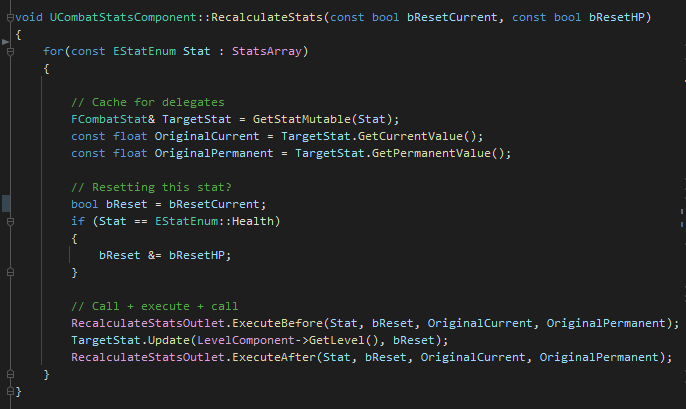
\includegraphics[scale=\ScreenshotScale]{recalculate-stats-code}
		\end{center}
		}
	\item{\textbf{\code{Outlet} arrays} are variables inside of \code{EffectableComponent}s. They hold \code{Outlet}s whose delegates execute when needed.
		\SubItem{\todo{Update this!} Let's use \code{StatsComponent}'s \code{AfterRecalculateStatsArray} in our example. In this case, after stats are recalculated (say, on level-up), the base PhA would increase by 10\% and the base SpA would decrease by 10\% (additively): }
		\begin{center}
			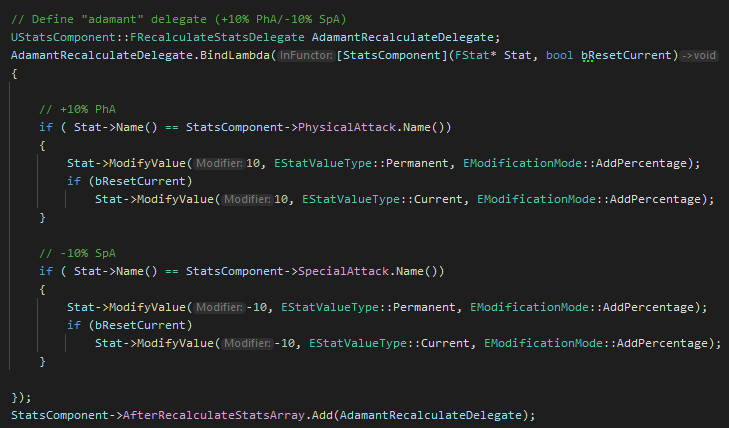
\includegraphics[scale=\ScreenshotScale]{adamant-code}
		\end{center}		 
		}
	\item{\textbf{\code{EffectComponent}s} are \code{ActorComponent}s that plug into \code{Outlet}s. These come in many forms, but an easy example is a \code{Buff}. \todo{Describe how this happens with pictures!}}
\end{itemize}

\sect{List of \code{EffectableComponent}s and \code{Outlet}s}

The following tables show all implemented \code{EffectableComponent}s and their delegate arrays. Note the ``base name'' indicates existence of:

\begin{enumerate}
	\item{the delegate signature \code{FBaseNameSignature};}
	\item{the private before/after arrays of \code{Outlet}s: \\\code{TArray<FBaseNameOutlet> BeforeBaseName}; and}
	\item{a function for each before/after to execute the arrays: \code{ExecuteBeforeBaseName (...)}.}
	\item{\code{AddBeforeBaseName}, a function to add an \code{Outlet} to the private array \code{BeforeBaseName} (which also puts it in the right order based on priority).}
\end{enumerate}

\noindent Note that the philosophy applies to what is \textit{probable} rather than what is \textit{possible}. Hence the list meant to be practical rather than exhaustive.

%--------------------------

\begin{longtblr}[
	caption = {\code{Outlet}s for \code{LevelComponent}},
	label = {delegate-arrays-levelcomponent},
]{
	colspec= {Q[l, wd=0.13\linewidth] Q[l, wd=0.35\linewidth] Q[l, wd=0.37\linewidth]},
	hline{1,Z} = {2pt},
}
	\todo{Todo}
	
\end{longtblr}

%--------------------------

\newcommand{\DelegateSpace}{\hspace*{1em}$\blacktriangleright$}
\newcommand{\DelegateNote}{\hspace*{2em}\textit{Note:}}

\begin{longtblr}[
	caption = {Delegate Arrays for \code{LevelComponent}},
	label = {delegate-arrays-levelcomponent},
]{
	colspec= {Q[l, wd=0.13\linewidth] Q[l, wd=0.72\linewidth]},
	hline{1,Z} = {2pt},
}

	%----------------------
	\hline
	\SetCell[c=2]{l}{\color{ICBlue}\textbf{GetBaseExpYield}}\\
	\hline
	\\
	%----------------------	
	
	\DelegateSpace{} Before	
		& {	\code{const float OriginalYield},\\
			\code{float\& ReturnedYield}}
		\\
		
		
	\DelegateSpace{} After	
		& {	\code{const float OriginalYield},\\
			\code{const float ReturnedYield}}
		\\
		
	%----------------------
	\hline
	\SetCell[c=2]{l}{\color{ICBlue}\textbf{GetCXP}}\\
	\hline
	\\
	%----------------------	

	\DelegateSpace{} Before			
		& {	\code{const uint32 OriginalCXP},\\ 
			\code{int32\& ReturnedCXP}}	
		\\ 
	\DelegateNote{}
		& \code{ReturnedCXP} is \code{int32\&} instead of \code{uint32\&} for Blueprint compatability.
		\\		
							
	\DelegateSpace{} After				
		& {	\code{const uint32 OriginalCXP}\\ 
			\code{const int32 ReturnedCXP}} 
		\\ 
	\DelegateNote{}
		& \code{ReturnedCXP} is \code{const int32} instead of \code{const uint32} for Blueprint compatability.
		\\
		
	%----------------------
	\hline
	\SetCell[c=2]{l}{\color{ICBlue}\textbf{GetExpYield}}\\
	\hline
	\\
	%----------------------	

	\DelegateSpace{} Before			
		& {	\code{const float OriginalYield},\\ 
			\code{float\& ReturnedYield},\\
			\code{const uint16 DefeatedLevel},\\
			\code{const uint16 VictoriousLevel}
			}\\
		\\
	\DelegateNote{}
		& ``Defeated'' and ``Victorious'' levels are provided for flexibility (e.g., in case you want to yield exp differently based on level difference, although technically you could always back-calculate the level difference based on the equation and \code{OriginalYield}).
		\\		
							
	\DelegateSpace{} After			
		& {	\code{const float OriginalYied},\\ 
			\code{const float ReturnedYield},\\
			\code{const uint16 DefeatedLevel},\\
			\code{const uint16 VictoriousLevel}
			}\\
		\\
	\DelegateNote{}
		& ``Defeated'' and ``Victorious'' levels are provided for symmetry with respect to the \code{Before} delegate (since \code{ReturnedValue} is already calculated, I can't think of why you would need them, but you never know!).
		\\
		
	%----------------------
	\hline
	\SetCell[c=2]{l}{\color{ICBlue}\textbf{GetMaxLevel}}\\
	\hline
	\\
	%----------------------	

	\DelegateSpace{} Before			
		& {	\code{const uint16 DefaultMax},\\ 
			\code{int32\& AttemptedMax}}	
		\\
	\DelegateNote{}
		& \code{DefaultMax} is defined in the code. It should normally be 100, but may change for certain subclasses (e.g., a \code{UBossLevelComponent} may have a max of 200 instead). Also, \code{AttemptedMax} is \code{int32\&} instead of \code{uint16\&} for Blueprint compatability.
		\\		
							
	\DelegateSpace{} After				
		& {	\code{const uint16 DefaultMax}\\ 
			\code{const int32 ReturnedMax}} 
		\\
		
	%----------------------
	\hline
	\SetCell[c=2]{l}{\color{ICBlue}\textbf{GetMinLevel}}\\
	\hline
	\\
	%----------------------	

	\DelegateSpace{} Before			
		& {	\code{const uint16 DefaultMin},\\ 
			\code{int32\& AttemptedMin}}	
		\\
	\DelegateNote{}
		& \code{DefaultMin} is defined in the code. It should normally be 1, but may change for certain subclasses (e.g., a \code{UEggLevelComponent} may have a min of 0 instead for whatever reason). Also, \code{AttemptedMin} is \code{int32\&} instead of \code{uint16\&} for Blueprint compatability.
		\\		
							
	\DelegateSpace{} After				
		& {	\code{const uint16 DefaultMin}\\ 
			\code{const int32 ReturnedMin}} 
		\\		
		
	%----------------------
	\hline
	\SetCell[c=2]{l}{\color{ICBlue}\textbf{SetBaseExpYield}}\\
	\hline
	\\
	%----------------------	

	\DelegateSpace{} Before			
		& {	\code{const float OldYield},\\ 
			\code{float\& AttemptedYield}}	
		\\		
							
	\DelegateSpace{} After				
		& {	\code{const float OldYield}\\ 
			\code{const float NewYield}} 
		\\
		
	%----------------------
	\hline
	\SetCell[c=2]{l}{\color{ICBlue}\textbf{SetCXP}}\\
	\hline
	\\
	%----------------------	

	\DelegateSpace{} Before			
		& {	\code{const uint32 OldCXP},\\ 
			\code{int32\& AttemptedCXP}}	
		\\
	\DelegateNote{}
		& \code{AttemptedCXP} is \code{int32\&} instead of \code{uint32\&} for Blueprint compatability.
		\\		
							
	\DelegateSpace{} After				
		& {	\code{const uint32 OldCXP}\\ 
			\code{const uint32 NewCXP}} 
		\\
	\DelegateNote{}
		& \code{UStatsComponent} subscribes to this in order to change stats on level change.
		\\
		
		
		
\end{longtblr}

%--------------------------

\begin{longtblr}[
	caption = {Delegate Arrays for \code{LevelComponent}},
	label = {delegate-arrays-levelcomponent},
]{
	colspec= {Q[l, wd=0.13\linewidth] Q[l, wd=0.72\linewidth]},
	hline{1,Z} = {2pt},
}

	%----------------------
	\hline
	\SetCell[c=2]{l}{\color{ICBlue}\textbf{RandomizeStats}}\\
	\hline
	\\
	%----------------------	
	
	\DelegateSpace{} Before	
		& {	
			\code{const EStatEnum TargetStat},\\
			\code{const FStatRandParams OriginalParams},\\
			\code{FStatRandParams\& ParamsToBeUsed}
		}
		\\
		
		
	\DelegateSpace{} After	
		& {	
			\code{const EStatEnum TargetStat},\\
			\code{const FStatRandParams OriginalParams},\\
			\code{const FStatRandParams UsedParams}
		}
		\\
		\DelegateNote{} 
			& The \code{EStatEnum} is not the acutal \code{FStat}. To get the \code{FStat} (such as \code{FHealth}), use \code{UStatsComponent::GetStat(EStatEnum)}.
		\\
		
	%----------------------
	\hline
	\SetCell[c=2]{l}{\color{ICBlue}\textbf{RecalculateStats}}\\
	\hline
	\\
	%----------------------	
	
	\DelegateSpace{} Before	
		& {	
			\code{const EStatEnum TargetStat},\\
			\code{const bool bResetCurrent},\\
			\code{const float OriginalCurrent},\\
			\code{const float OriginalPermanent}
		}
		\\
		
		
	\DelegateSpace{} After	
		& {	
			\code{const EStatEnum TargetStat},\\
			\code{const bool bResetCurrent},\\
			\code{const float OriginalCurrent},\\
			\code{const float OriginalPermanent}
		}
		\\
			
		
	
\end{longtblr}

%====================================================

\sect{Making Your Own \code{Outlet}}

As an example, let's use \code{GetBaseExpYield}. (You can imagine that this is an important \code{Outlet} for tweaking levelling curves.) Here's what to do:\\

\begin{enumerate}
	\item{\textbf{Plan ahead.} I would sincerely recommend you writing down what parameters your \code{Outlet} \code{Before} and \code{After} delegates take on paper. We go to a few files and it's easy to be inconsistent.}
	\item{\textbf{Go to the right directory.} We want to place the \code{Outlet} inside of \code{ULevelComponent}, so we'll start with that directory. If yours doesn't contain an ``Outlets'' directory, create one and place your \code{Outlet}(s) there.}
	\item{\textbf{Copy + paste file.} The easiest way is to copy + paste pre-existing \code{Outlet}s. In this example, we'll copy + paste \code{SetCXPOutlet.h} and name the new file \code{GetBaseExpYield.h}. \\
	\begin{center}
		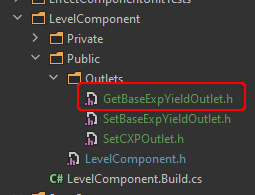
\includegraphics[scale=\ScreenshotScale]{create-outlet-rename}
	\end{center}
	\noindent \textit{Note: this includes both \code{BeforeGetBaseExpYield} and \code{AfterGetBaseExpYield} functionality. You don't have to make two different files!}
	}
	\item{\textbf{Replace old name.} Open the new file and you'll still see the base name ``SetCXP'' everywhere. The easiest way is to do a find+replace ``SetCXP'' $\rightarrow$ ``GetBaseExpYield''. This replaces everything from the \code{.generated} include to the delegate signatures. If you're curious, you can look more in-depth and replace instances one-by-one.}
	\item{\textbf{Declare delegate signatures.} In this case, we want the \code{Before} delegate signature to take two arguments: the original, unmodified yield and the one that will be returned from the \code{GetBaseExpYield} function.\\
	\begin{center}
		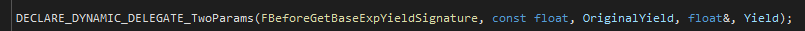
\includegraphics[scale=\ScreenshotScale]{create-outlet-signature}
	\end{center}
	You should also set the \code{After} signature in the same manner. \textit{Note: yours might use more than two parameters or different parameter types. Modify accordingly.}
	}
	\item{\textbf{Declare \code{Outlet} functions.} In order to be able to call \code{ExecuteBefore} on your \code{Outlet}, you need to tell it a few things. The figure below displays a few things in red you should look at:\\
	\begin{center}
		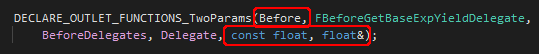
\includegraphics[scale=\ScreenshotScale]{create-outlet-functions}
	\end{center}
		\begin{itemize}
			\item{Whether it's a \code{Before} or \code{After} type \code{Outlet}. This affects execution based on priority:
			\begin{tcolorbox}[colback=gray!20!white,colframe=blue!75!black,title=Priorities]
			
				The lower the priority, the farther away it is from execution. If two priorities are tied, the older effect is executed first. Order is set externally by \code{UEffectsComponent} \todo{fact check this}. Order:\\
				\begin{itemize}
					\item{Intrinsic \code{Before} delegates (no \code{UEffect} affiliated)}
					\item{\code{Before} delegates:
						\begin{itemize}
							\item{Priority 1}
							\item{Priority 2.a (older)}
							\item{Priority 2.b (newer)}
							\item{...}
						\end{itemize}
						}
					\item{[Function executes]}
					\item{\code{After} delegates:
						\begin{itemize}
							\item{...}
							\item{Priority 2.b (newer)}
							\item{Priority 2.a (older)}
							\item{Priority 1}
						\end{itemize}
						}
					\item{Intrinsic \code{After} delegates (have the final say)}
				\end{itemize}
				
			As an example, consider two delegates: one that says you can't take damage no matter what (call the \code{UBuff} ``Invincible'') and another that says damage against you can't be avoided no matter what (call the \code{UDebuff} ``Weakened''). What happens when the target takes damage? Well, it depends on priority:
			\begin{itemize}
				\item{They're probably subscribed to the \code{Before} delegate in \code{UStatsComponent} called \code{ModifyStatOutlet} with the target \code{FStat} being \code{Health}.}
				\item{Note that they're both \code{Before} delegates.}
				\item{Let's say Invincible has Priority 100 and Weakened has Priority 150. The result is the target takes damage because:
					\begin{enumerate}
						\item[1)]{Invincible first sets the damage to zero.}
						\item[2)]{Weakened then sets the damage to no less than its original value.}
					\end{enumerate}
				}
				\item{If Weakened has lower Priority, the result is flipped and the target takes no damage.}
			\end{itemize}
	 
	 \end{tcolorbox}\vspace*{12pt}
			}
			\item{The parameters you defined in the delegate's signature. I know, I know---anytime you repeat code, you're probably doing something wrong. The biggest issue here is the UHT. The main (but not only) issue is that you can't have \code{UPROPERTY}s inside macros or the property won't register. If you have a better way of automating this, \textit{tell me!}}
			\item{Don't forget the \code{After} variant's delegates, which should probably be \code{const}.}
		\end{itemize}
	}
	\item{\textbf{Check number of parameters.} I make a point of this because I find it's my most common error. Make sure your declared signature \textit{and} declared \code{Outlet} function macros have the correct number of params (two in our case). Explicitly, you might need to use \code{DECLARE\_DYNAMIC\_DELEGATE\_FourParams(...)}.}
	\item{\textbf{Declare \code{UPROPERTY}.} Inside the \code{UEffectableComponent} (in this example, \code{ULevelComponent}), declare the \code{Outlet} as a variable. Note that it's custom to have this \code{UPROPERTY} as public and in the ``Outlets'' category. It's also a good idea to comment the \code{UPROPERTY} with the parameters.
	\begin{center}
		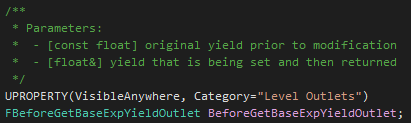
\includegraphics[scale=\ScreenshotScale]{create-outlet-uproperty}
	\end{center}
	
	\textit{Note:} I use Rider, so it imports \code{\#include}s automatically. Make sure yours does, too.
	}
	\item{\textbf{Implement.} Now it's time to place your \code{Outlet} in the appropriate place(s). For our example, it's pretty simple: place it inside of \code{GetBaseExpYield} in \code{ULevelComponent}'s \code{.cpp} file.
	\begin{center}
		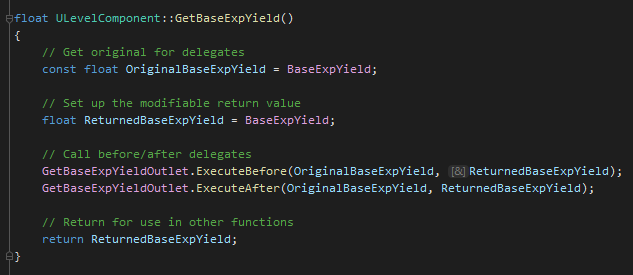
\includegraphics[scale=\ScreenshotScale]{create-outlet-cpp}
	\end{center}
	Note that you might have to do things like cache original values.
	}
	\item{\textbf{A note on complementary delegates.} If you create a \code{Before} \code{Outlet}, you should also create an \code{After} \code{Outlet}. The biggest difference might be the delegate signature (e.g., reference ``\code{\&}'' to \code{const}).
			
	An example where this would be necessary is an animation delegate. You only want to fire a ``bonus exp'' animation \textit{after} the amount of exp has been determined, checked, and is now constant.
	
	In some cases, it may not be necessary to have both \code{Before} and \code{After} delegates in a function. If you want only one delegate type, or three, or ten, the system is flexible enough to handle it. However, it's recommended to K.I.S.S.
	}
\end{enumerate}

\sect{Making Your Own Effects}

Suppose you want to make your own effect from scratch. \todo{todo}

\end{document}